\documentclass{article}
\usepackage[utf8]{inputenc} % åäö
\usepackage{tikz}
\usetikzlibrary{calc, fit, shapes.geometric, arrows, decorations.pathmorphing, positioning, fit, matrix, backgrounds}
\pgfdeclarelayer{background}
\pgfdeclarelayer{foreground}
\pgfsetlayers{background,main,foreground}
\usepackage[T1]{fontenc}


\tikzstyle{startstop} = [rectangle, rounded corners, minimum width=3cm, minimum height=1cm,text centered, draw=black, fill=red!30]

\tikzstyle{io}       = [trapezium, trapezium left angle=75, trapezium right angle=105, minimum width=2cm, minimum height=1cm, text centered, draw=black, fill=blue!30]
\tikzstyle{process}  = [rectangle, minimum width=2cm, minimum height=2cm, text centered, draw=black, fill=orange!30]
\tikzstyle{decision} = [diamond,   minimum width=2cm, minimum height=2cm, text centered, draw=black, fill=green!30]
\tikzstyle{arrow}    = [-open triangle 45]
\tikzstyle{dotbox}   = [draw, dotted, rectangle, rounded corners]

\newcommand*{\prim}{\ensuremath{\prime}}

\begin{document}






\section{Aspects of transformation engines}

\begin{tabular}{r | c | c}
  & \textbf{Generalized output} & \textbf{Specialized output} \\ \hline

  \textbf{Generalized input} &
  A
  &
  B 

  \\ \hline

  \textbf{Specialized input} &
  C
  &
  D
\end{tabular}







\paragraph{Input, output}

\begin{tabular}{r | c | c }
  &
  \textbf{Input} &
  \textbf{Output}
  \\ \hline

  Type A &
  s &
  s \\ \hline

  Type B &
  G &
  s \\ \hline


  Type C &
  s &
  G \\ \hline

  Type D &
  G &
  G \\ \hline

\end{tabular}










\paragraph{Input, output, config}

\begin{tabular}{l | c | c | c}
  &
  \textbf{Input} &
  \textbf{Output} &
  \textbf{Config}
  \\ \hline

  Type A\prim &
  s &
  s &
  s \\ \hline

  Type A\prim\prim &
  s &
  s &
  G \\ \hline



  Type B\prim &
  G &
  s &
  s \\ \hline

  Type B\prim\prim &
  G &
  s &
  G \\ \hline



  Type C\prim &
  s &
  G &
  s \\ \hline

  Type C\prim\prim &
  s &
  G &
  G \\ \hline



  Type D\prim &
  G &
  G &
  s \\ \hline

  Type D\prim\prim &
  G &
  G &
  G \\ \hline

\end{tabular}





\subsection{Specialized in, Specialized out (Quadrant D)}
i.e. LaTeX to pdf converter.

\begin{figure}[h]
  \centering

  \begin{tikzpicture}[node distance=3cm]
  \node (trans)  [startstop, right of=input, align=center, xshift=2cm] {
    Specialized \\\\

    \begin{tikzpicture}
      \node (input)  [io] {Input};
      \node (engine) [process, right of=input, xshift=2cm] {Transformation engine};
      \node (output) [io,      right of=engine, xshift=2cm] {Output};
      \node (conf)   [io,      above of=engine]{Configuration};

      % arrows
      \draw [arrow] (input)  -- (engine);
      \draw [arrow] (engine) -- (output);
      \draw [arrow] (conf)   -- (engine);
    \end{tikzpicture}
  };
  \end{tikzpicture}

  \caption{Specialized in, Specialized out.}
\end{figure}





\subsection{Specialized in, Generalized out (Quadrant C)}
E.g. XML combined with XSLT. TODO.

\begin{figure}[h]
  \centering

  \begin{tikzpicture}[node distance=3cm]
  \node (trans)  [startstop, right of=input, align=center, xshift=2cm] {
    Specialized \\\\

    \begin{tikzpicture}
      \node (input)  [io] {Input};
      \node (engine) [process, right of=input, xshift=2cm] {Transformation engine};
      \node (conf)   [io,      above of=engine]{Configuration};

      \draw [arrow] (input)  -- (engine);
      \draw [arrow] (conf)   -- (engine);
    \end{tikzpicture}
  };
  \node (output) [io,      right of=trans, xshift=4cm] {Output};

  % arrows
  \draw [arrow] (trans) -- (output);
  \end{tikzpicture}

  \caption{Specialized in, Generalized out.}
\end{figure}






\subsection{Generalized in, Specialized out (Quadrant B)}
This is an interesting set of transformation programs that, in theory, can take any input, but always converts the output to a fixed kind of output. For some reason the transformation engine is fixed to that type, and it would be significantly costly to rewrite the transformation program to accommodate a new format.


\begin{figure}[h]
  \centering

  \begin{tikzpicture}[node distance=3cm]
    \node (input)  [io, left of=trans] {Input};
    \node (trans)  [startstop, right of=input, align=center, xshift=3cm] {
    Specialized \\\\

    \begin{tikzpicture}
      \node (engine) [process, right of=input, xshift=2cm] {Transformation engine};
      \node (conf)   [io,      above of=engine]{Configuration};
      \node (output) [io,      right of=trans, xshift=3cm] {Output};

      \draw [arrow] (conf)   -- (engine);
      \draw [arrow] (engine) -- (output);
    \end{tikzpicture}
  };

  % arrows
  \draw [arrow] (input)  -- (trans);
  \end{tikzpicture}

  \caption{Generalized in, Specialized out.}
\end{figure}







\subsection{Generalized in, Generalized out (Quadrant A)}
These are transformation engines that are prepared for taking general input, and providing facilities to give general output. An example program that exhibits this behavior is the all-mighty pandoc library.

\begin{figure}[h]
  \begin{tikzpicture}[node distance=3cm]
  \node (input)  [io] {Input doc};
  \node (engine) [process, right of=input, xshift=1cm] {Transformer};
  \node (trans)  [startstop, above of=engine, align=center] {
    Specialized \\\\

    \begin{tikzpicture}
      \node (conf) [io]{Conf};
    \end{tikzpicture}
  };
  \node (output) [io,      right of=engine, xshift=1cm] {Output doc};

  % arrows
  \draw [arrow] (input)  -- (engine);
  \draw [arrow] (engine) -- (output);
  \draw [arrow] (trans)   -- (engine);
  \end{tikzpicture}

  \caption{Generalized in, Generalized out.}
\end{figure}












\section{A third dimension}
\begin{tabular}{l c c c}
&
\textbf{Input}  &
\textbf{Output} &
\textbf{Config} \\
\hline

Generalized
\\
Specialized

\end{tabular}





\begin{tabular}{c c c}

\begin{tabular}{c}
Generalized input
\\ \hline
Specialized input
\end{tabular}

&

\begin{tabular}{c}
Generalized output
\\ \hline
Specialized output
\end{tabular}

&

\begin{tabular}{c}
Generalized config
\\ \hline
Specialized config
\end{tabular}

\end{tabular}







\section{Arbitrary language with XML \& XSLT}
\begin{itemize}
\item \textbf{Coupling to output format} Since the transformer transforms to XML,We have coupled ourselves to the XML language and thus need to rewrite the transformation engine if something new would come along.
\item \textbf{Little control may cause extra work} The level of control that the user have on the intermediate format is utterly dependent on the level of control the transformation engine expose in the transformation configuration file. If a configuration file even exist. If it does not, or offer a low level of control, and the transformation engine by default spits out some utterly verbose format in a completely different way than we might imagine -- well, then, in the next step we might have to jump through a bunch of serious hoops with our transformations (to get rid of all this ``blabber'') in order to reach the end format we actually want to achieve. 
\item \textbf{Coupling to input format} Since the transformation engine is written with the intent of transforming content written in format F to XML, if another person need a transformer that transforms from format F' to XML, well then tant pis, we need to write another transformer engine.
\end{itemize}







\section{fooo}

\begin{figure}[p]
  \centering

  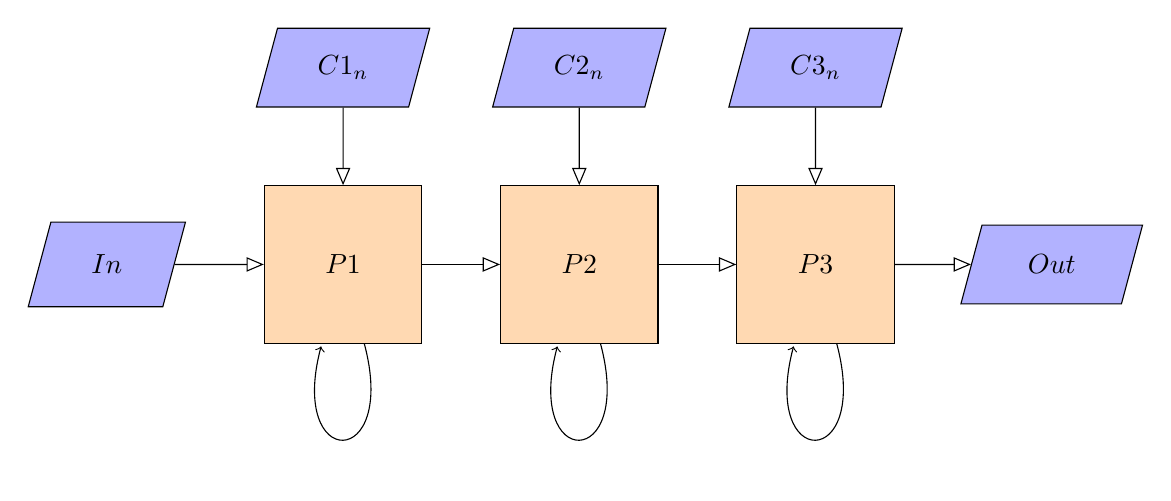
\begin{tikzpicture}[node distance=.5cm]
    \node (in)  [io]                                 {\(In\)};
    \node (P1)  [process, right of=in, xshift=2.5cm] {\(P1\)};
    \node (P2)  [process, right of=P1, xshift=2.5cm] {\(P2\)};
    \node (P3)  [process, right of=P2, xshift=2.5cm] {\(P3\)};
    \node (out) [io,      right of=P3, xshift=2.5cm] {\(Out\)};
    \node (C1)  [io,      above of=P1, yshift=2cm] {\(C1_n\)}; % {Semantics};
    \node (C2)  [io,      above of=P2, yshift=2cm] {\(C2_n\)}; % {Derivations};
    \node (C3)  [io,      above of=P3, yshift=2cm] {\(C3_n\)}; % {Presentation};




    \draw [arrow] (in) -- (P1);
    \draw [arrow] (P1) -- (P2);
    \draw [arrow] (P2) -- (P3);
    \draw [arrow] (P3) -- (out);
    \draw [arrow] (C1) -- (P1);
    \draw [arrow] (C2) -- (P2);
    \draw [arrow] (C3) -- (P3);
    \draw [arrow] (P1) edge[loop below]();
    \draw [arrow] (P2) edge[loop below]();
    \draw [arrow] (P3) edge[loop below]();
    %\path [line]  (P3) edge[P3 right];



    % \begin{pgfonlayer}{background}
    %   \node [dotbox, fit={(conf) (input)}]{};
    % \end{pgfonlayer}

  \end{tikzpicture}

  \caption{Suggested ideal refinement of a Quadrant A program.}
  \label{fig:workflows-framework-gen-in-gen-out}
\end{figure}









\end{document}
